\chapter{免疫系統}
\chapterauthor{邱柏偉}

\section{摘要}
免疫系統(Immune System)為我們抵擋入侵的外來病原體(細菌和病毒),使我們免受於病痛的侵擾,現在就讓我們來看看免疫系統到底是怎麼運作的吧!!!
\section{免疫細胞的種類}
在我們的體內有一群專門負責抵抗病原體的細胞,它們就是白血球(leukocytes)。因此,接下來我們就來看看白血球又分為哪些種類吧!
\begin{enumerate}
\item 顆粒性白血球
	\begin{enumerate}
	\item 嗜中性球(Neutrophil Granulocytes):
		\begin{enumerate}
		\item 占人體內白血球約65\%~70\%
		\item 感染時做\underline{\hspace{2cm}},可\underline{\hspace{2cm}}病原體
		\end{enumerate}
	\item 嗜酸性球(Eosinophil Granulocytes):
		\begin{enumerate}
		\item 占人體內白血球約2\%~4\%
		\item 吞噬功能有限
		\item 發生過敏反應的時候,產生\underline{\hspace{2cm}}$\rightarrow$減輕過敏症狀
		\item 被寄生蟲感染時,嗜酸性球會附著在其表面,釋出破壞性酵素
		\end{enumerate}
	\item 嗜鹼性球(Basophil Granolucytes):
		\begin{enumerate}
		\item 占人體內白血球約<0.5\%
		\item 在特殊情形下會釋放出其內含的\underline{\hspace{2cm}}(Histamine)\\
		$\rightarrow$引起各種\underline{\hspace{2cm}}和使血管擴張(\underline{\hspace{2cm}})

		\end{enumerate}
	\end{enumerate}
\item 淋巴球(Lymphocytes):
	\begin{enumerate}
	\item T細胞(T Cells):
		\begin{enumerate}
		\item T細胞的表面有各種可以跟\underline{\hspace{2cm}}結合的專一性受體,能辨識不同
		\end{enumerate}
	\item B細胞(B Cells):
		\begin{enumerate}
		\item 能分泌\underline{\hspace{2cm}}(Antibody),又稱\underline{\hspace{2cm}}(Immunoglobin)
		\end{enumerate}
	\end{enumerate}

\end{enumerate}
\section{免疫反應}
用說的太麻煩了,我們來玩個遊戲來幫助我們了解免疫反應吧!

\section{講師介紹}
\begin{itemize}
\item 姓名:邱柏偉
\item 性別:男
\item 特色:在高一時參加生物奧林匹亞徵選,僅以一題之差落選,令人惋惜、每天都會帶著Campbell往返學校及家中(編按:Campbell為普通生物學的經典教材,精裝版一冊重達2公斤)、會對經過的熟人說小恐龍(編按:可試著對講師說小恐龍,可能會有驚喜喔)、最近為了貼補家用,兼職蜂農。
\item 名言:你是小恐龍、這題真的很小恐龍耶、小恐龍。
\end{itemize}

\begin{figure}[H]
\graphicspath{{biology/}}
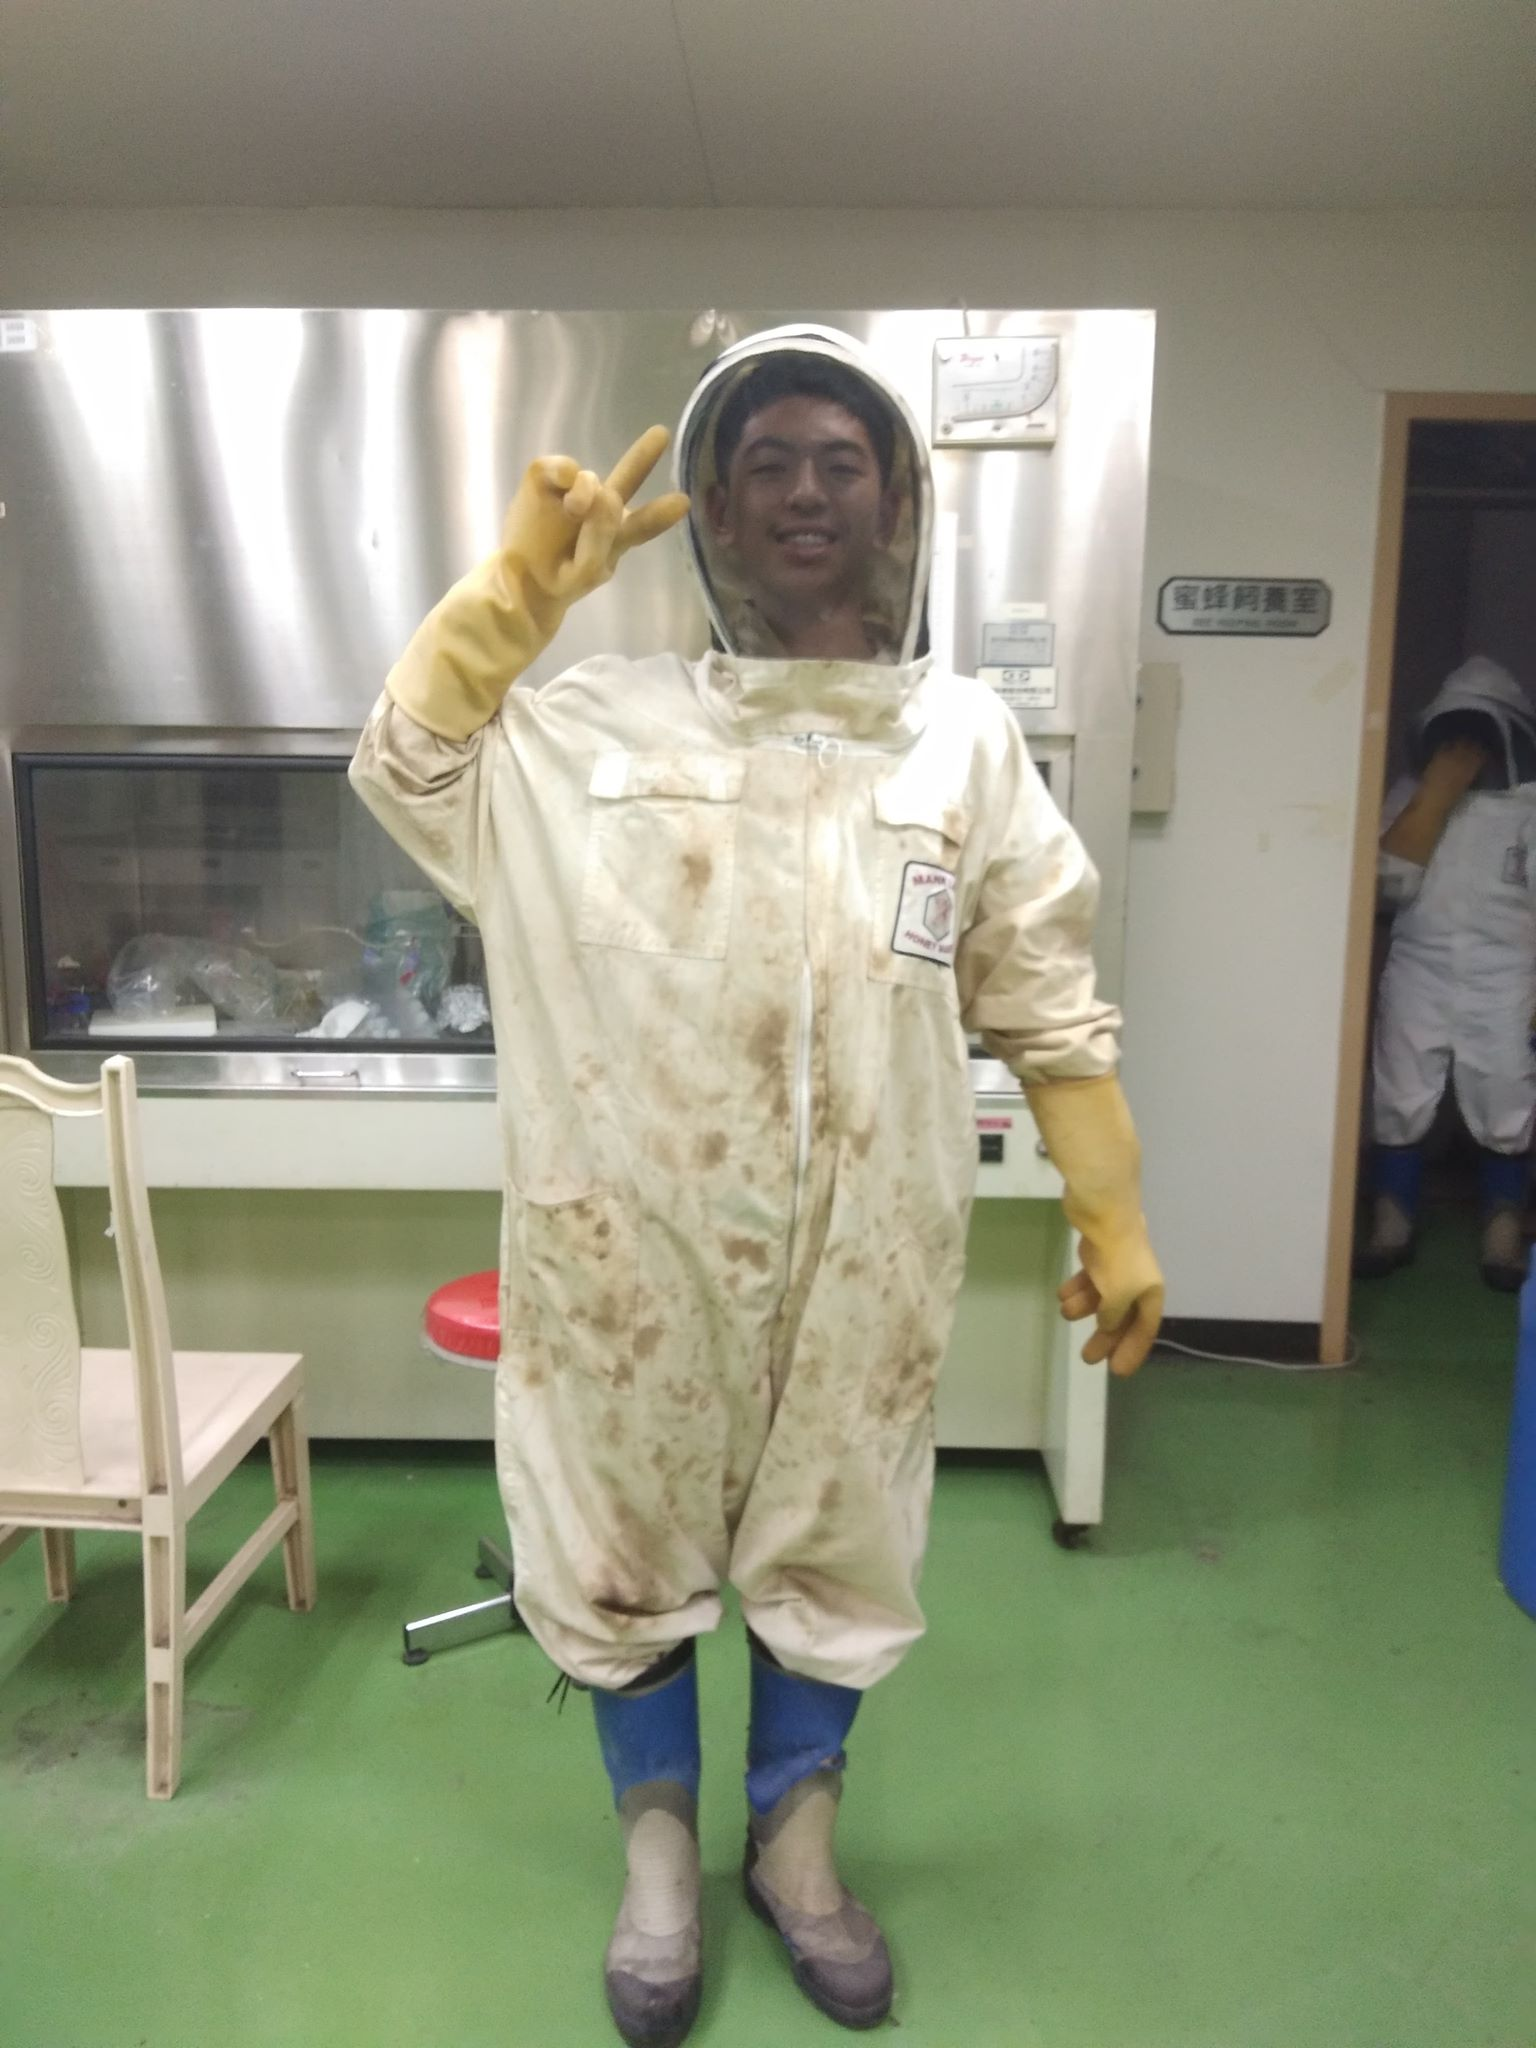
\includegraphics[width=8cm, center]{farmer.jpg}
\caption{蜂農} \vskip 10 pt
\label{fig:farmer}
\end{figure}